
In this chapter, we present the methodology that we are
proposing for learning chunks of good designs. We introduce a  
design optimization problem, the brushless DC permanent magnet motor 
design problem, and apply our methodolgy on this problem as we 
elucidate each step. The brushless DC permanent magnet design problem 
was first analyzed in \cite{chidambaram1999} as an illustration of a 
new catalog-based customization procedure. The same problem 
was analyzed in \cite{deb2008} to discover 
innovative design principles from the optimization results. We borrow 
the same problem formulation as in \cite{deb2008} for our study.

\section{Overview of the chunking process}
Figure \ref{overview} shows the steps of our proposed chunking 
process. The first stage in the process is obtaining a set of optimal 
solutions using multi-objective optimization. The second step is the 
manifold estimation of the optimal solutions obtained in the first 
step. The next step, clustering the optimal solutions, is the most
important step in chunking procedure. In this step the optimal 
solutions are clustered using a density based clustering algorithm in 
the combined objective-parameter space space. Finally we model the 
clusters into manifolds which represent the chunks of similar 
optimal solutions.
 
\begin{figure}[ht]\begin{center}
 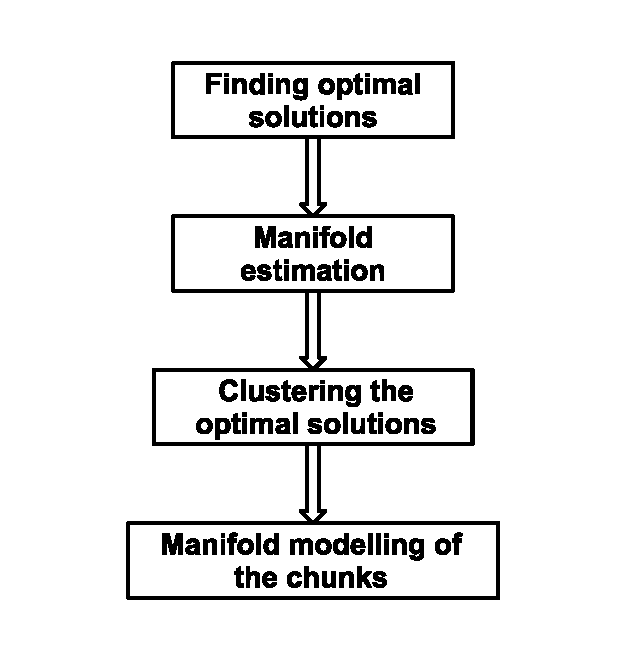
\includegraphics[width=75mm, height=75mm]{dia/overview.eps}
 \caption{Overview of the chunking process}
 \label{overview}
\end{center}\end{figure}



\section{Obtaining set of optimal designs}
Since we want to learn chunks of ``good" solutions we must have a way 
of characterising good solutions. In context of design, only the best
possible designs may be considered as good, a designer who produces 
feasible but sub-optimal designs can not be called an expert. A human 
designer during her routine exploration of a design problem comes 
across some designs that are superior to all others. These are the 
designs that she is more likely to retain in her memory as a chunk. In
effect, she is searching for optimal designs which when found are 
retained. The first step of our procedure to learn patterns of good 
designs is to obtain a representative set of such optimal designs.  
In this section, we discuss the possible techniques of obtaining such 
representative optimal solutions set.

\subsection{Conventional multi-objective optimization techniques}
In classical multi-objective optimization techniques the objectives 
are combined to form one single objective using some knowledge of the 
problem being solved. The optimization of the single objective-results
in a single pareto-otimal solution.

One of the classical methods of multi-objective optimization is the 
method of objective weighting \cite{deb2001,deb1994}. 
Multiple objectives are combined into an overall objective by 
assigning fractional weights to the individual objective functions 
which sum to one. The optimal solution is controlled by the weight 
vector. 

In the method of distance functions, the single objective is derived
from multiple objectives using a demand level vector 
$\overline{\textbf{y}}$ as follows:

\begin{align}
Z = \left[ \displaystyle\sum\limits_{i=1}^N {|f_i(\textbf{x} - \overline{y_i})|}\right] ^{1/r}, \quad &1 \leqslant r < \infty 
\end{align}

where $\textbf{x} \in \textbf{X}$, the feasible region. An arbitrary 
demand level vector may result in a objective that doesn't  have an 
optimal solution, hence the decision maker must have a thorough
knowledge of individual optima of each objective prior to the 
selection of the demand level.

The Min-Max formulation method is different in principle from the 
above two methods in that it attempts to minimize the relative 
deviations from the individual optima, that is to say, it tries to 
minimize the objective conflict.

The most important drawback of these classical multi-objective 
optimization methods with respect to our objective is that they yeild
only one pareto-optimal solution in a single run. Secondly, all of 
them require some knowledge of the problem, such as the weight vector
or demand vector. Moreover it is not possible to find all 
pareto-optimal solutions in some non-convex multi-objective optimization
problems.

\subsection{Evolutionary algorithms for multi-objective optimization}
Evolutionary approaches to multi-objective optimization are much more
suited to the purpose of generating a representative optimal solution 
sets, as they can search the solution space in parallel for optimal 
solutions , and produce a set of pareto-optimal solutions in a
single run. 

Evolutionary algorithms try to mimic the process of natural selection,
whereby only the specimen most adapted to the environment survive and
evolve. All the algorithms start with randomly chosen feasible 
population and search and reproduce the best solutions in the 
population. This search and reproduce procedure is repeated for
many generations, until the next generation doesn't result in 
significant improvement. The first practical evolutionary 
multi-objective optimization algorithm was the Vector Evaluated 
Genetic Algorithm (VEGA) \cite{schaffer1985}. One of the problems with
VEGA is its bias towards some pareto-optimal solutions. A 
non-dominated sorting procedure was proposed by Goldberg to overcome 
this drawback, in which a ranking selection method is used to 
emphasize good points and a niche method is used to maintain stable 
sub-populations of good points. One algorithm that that implements 
this non-dominated sorting procedure is the NSGA 
\cite{deb1994}.

This algorithm was further improved upon, and a new algorithm 
NSGA-II \cite{deb2002} was proposed which had better and faster 
convergence towards the true pareto-front due to a fast non-dominated
sorting approach. Since it was first proposed, the NSGA-II has found
application in a wide variety of engineering optimizations and design 
problems. Several studies have been published illustrating the 
versatility of NSGA-II in a wide variety of situations. All these 
advantages that NSGA-II has over other algorithms, and its proven
versatility make it an ideal candidate for the purpose of generating 
a set of pareto-optimal solutions 

\subsection{The BDCPM motor design problem}
We now introduce the BDCPM (brushless DC permanent magnet motor) 
design problem and derive a set of pareto-optimal solutions using 
NSGA-II. A BDCPM motor comprises of an outer stator assembly with 
windings on a frame  and inner rotor assembly having pemanently 
mounted magnets, shown in Figures \ref{bdcpmStator} and 
\ref{bdcpmRotor}. Several variants of this basic design exist. The 
original study \cite{chidambaram1999} considered 24 slots 4 pole 
machine.


\subsubsection{The multi-objective optimization problem}
Figure \ref{bdcpmRotor} shows the rotor assembly of a BDCPM motor. A
ring-magnet is bonded onto a stepped shaft that fits in the bore of
the stator assembly. The total length of the motor is $L_{sh}$. The 
shaft length is equal to the sum of stack length and the side 
clearances, $ L_{sh} = L + 2L_{cl}$. The side clearance values, 
$L_{cl}$ are listed in Table \ref{ltypeDimTable}.

\begin{figure}[ht]\begin{center}
 \fbox{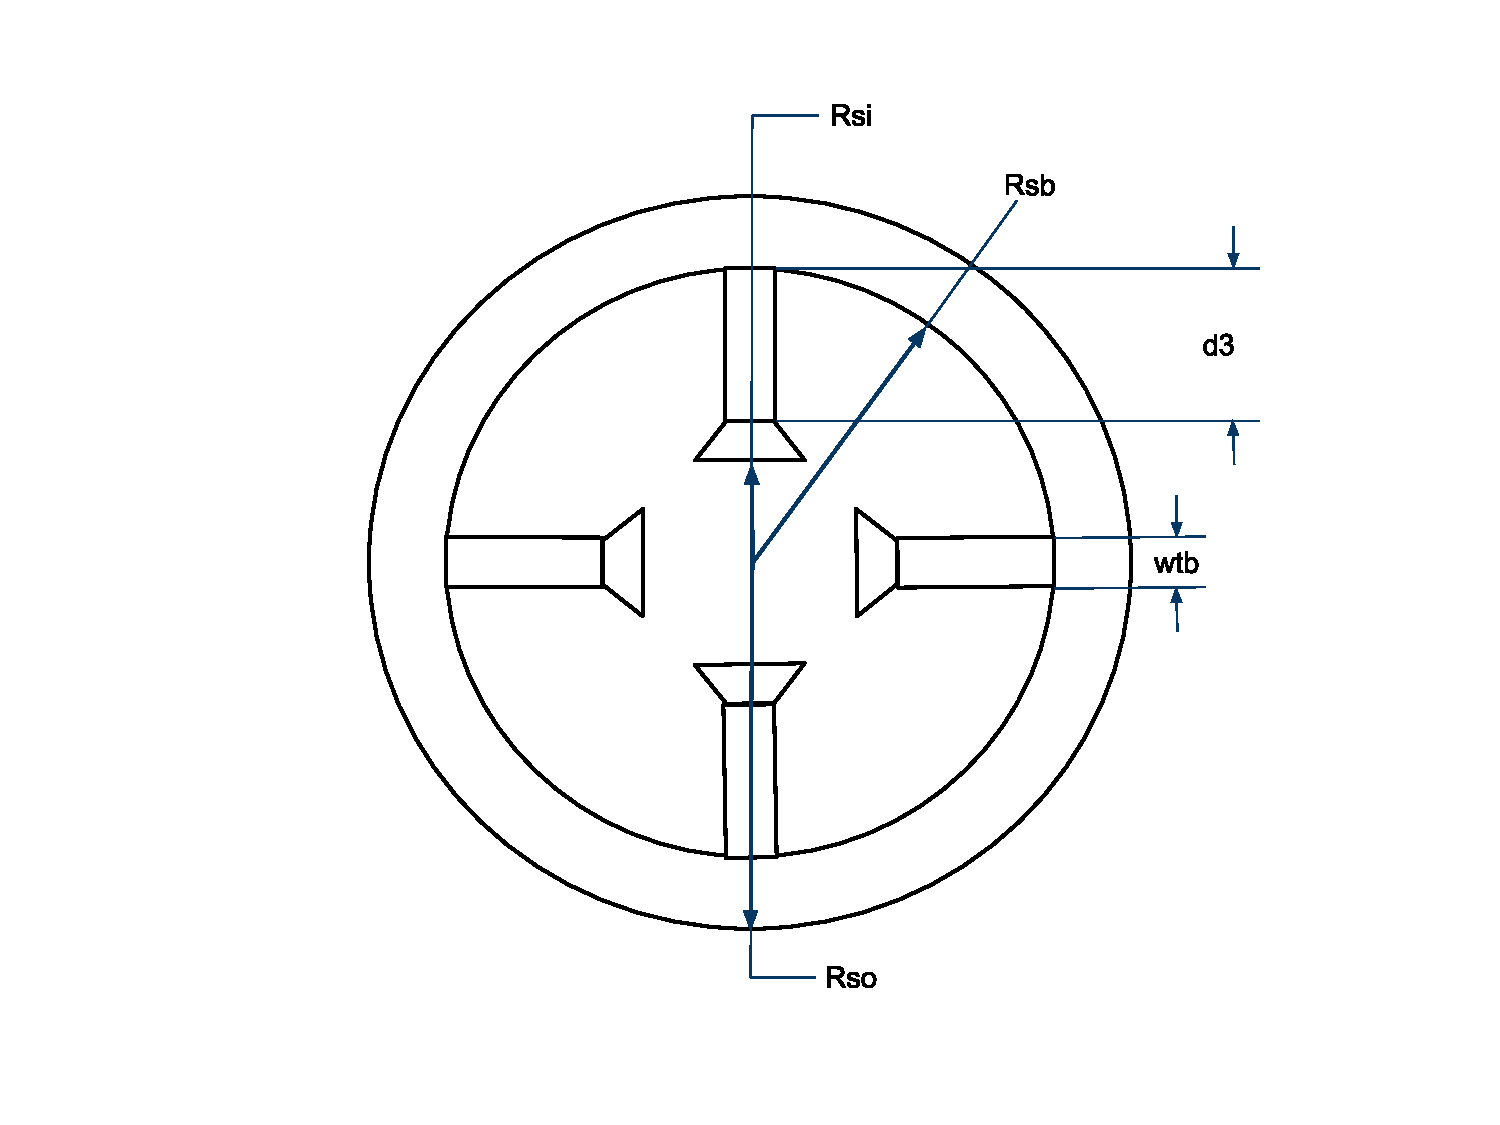
\includegraphics[width=100mm, height=75mm]{diagrams/bdcpmStator.eps}}
 \caption{BDCPMM Stator assembly}
 \label{bdcpmStator}
\end{center}\end{figure}

\begin{table}[!ht]
\centering
\begin{tabular}{|c|c|c|c|c|c|c|c|}
 \hline
 $L_{type}$ & $R_{si}$ (mm.) & $d_3$ (mm.) & $w_{tb}$ (mm.) & $w_{bi}$ (mm.) & $L_{cl}$ (mm.)& $R_{sh}$ (mm.) & $R_{st}$ (m) \\
 \hline
 X & 21.90 & 12.0 & 2.39 & 5.23 & 4.215 & 4.11 & 0.016 \\
 \hline
 Y & 22.22 & 15.1 & 2.39 & 5.23 & 4.265 & 4.11 & 0.016 \\
 \hline
 Z & 25.40 & 15.1 & 2.80 & 5.50 & 4.775 & 4.45 & 0.019 \\
 \hline
 \end{tabular}
\caption{Dimensions of the BDCPM motor family}
\label{ltypeDimTable}
\end{table}

\begin{figure}[ht]\begin{center}
 \fbox{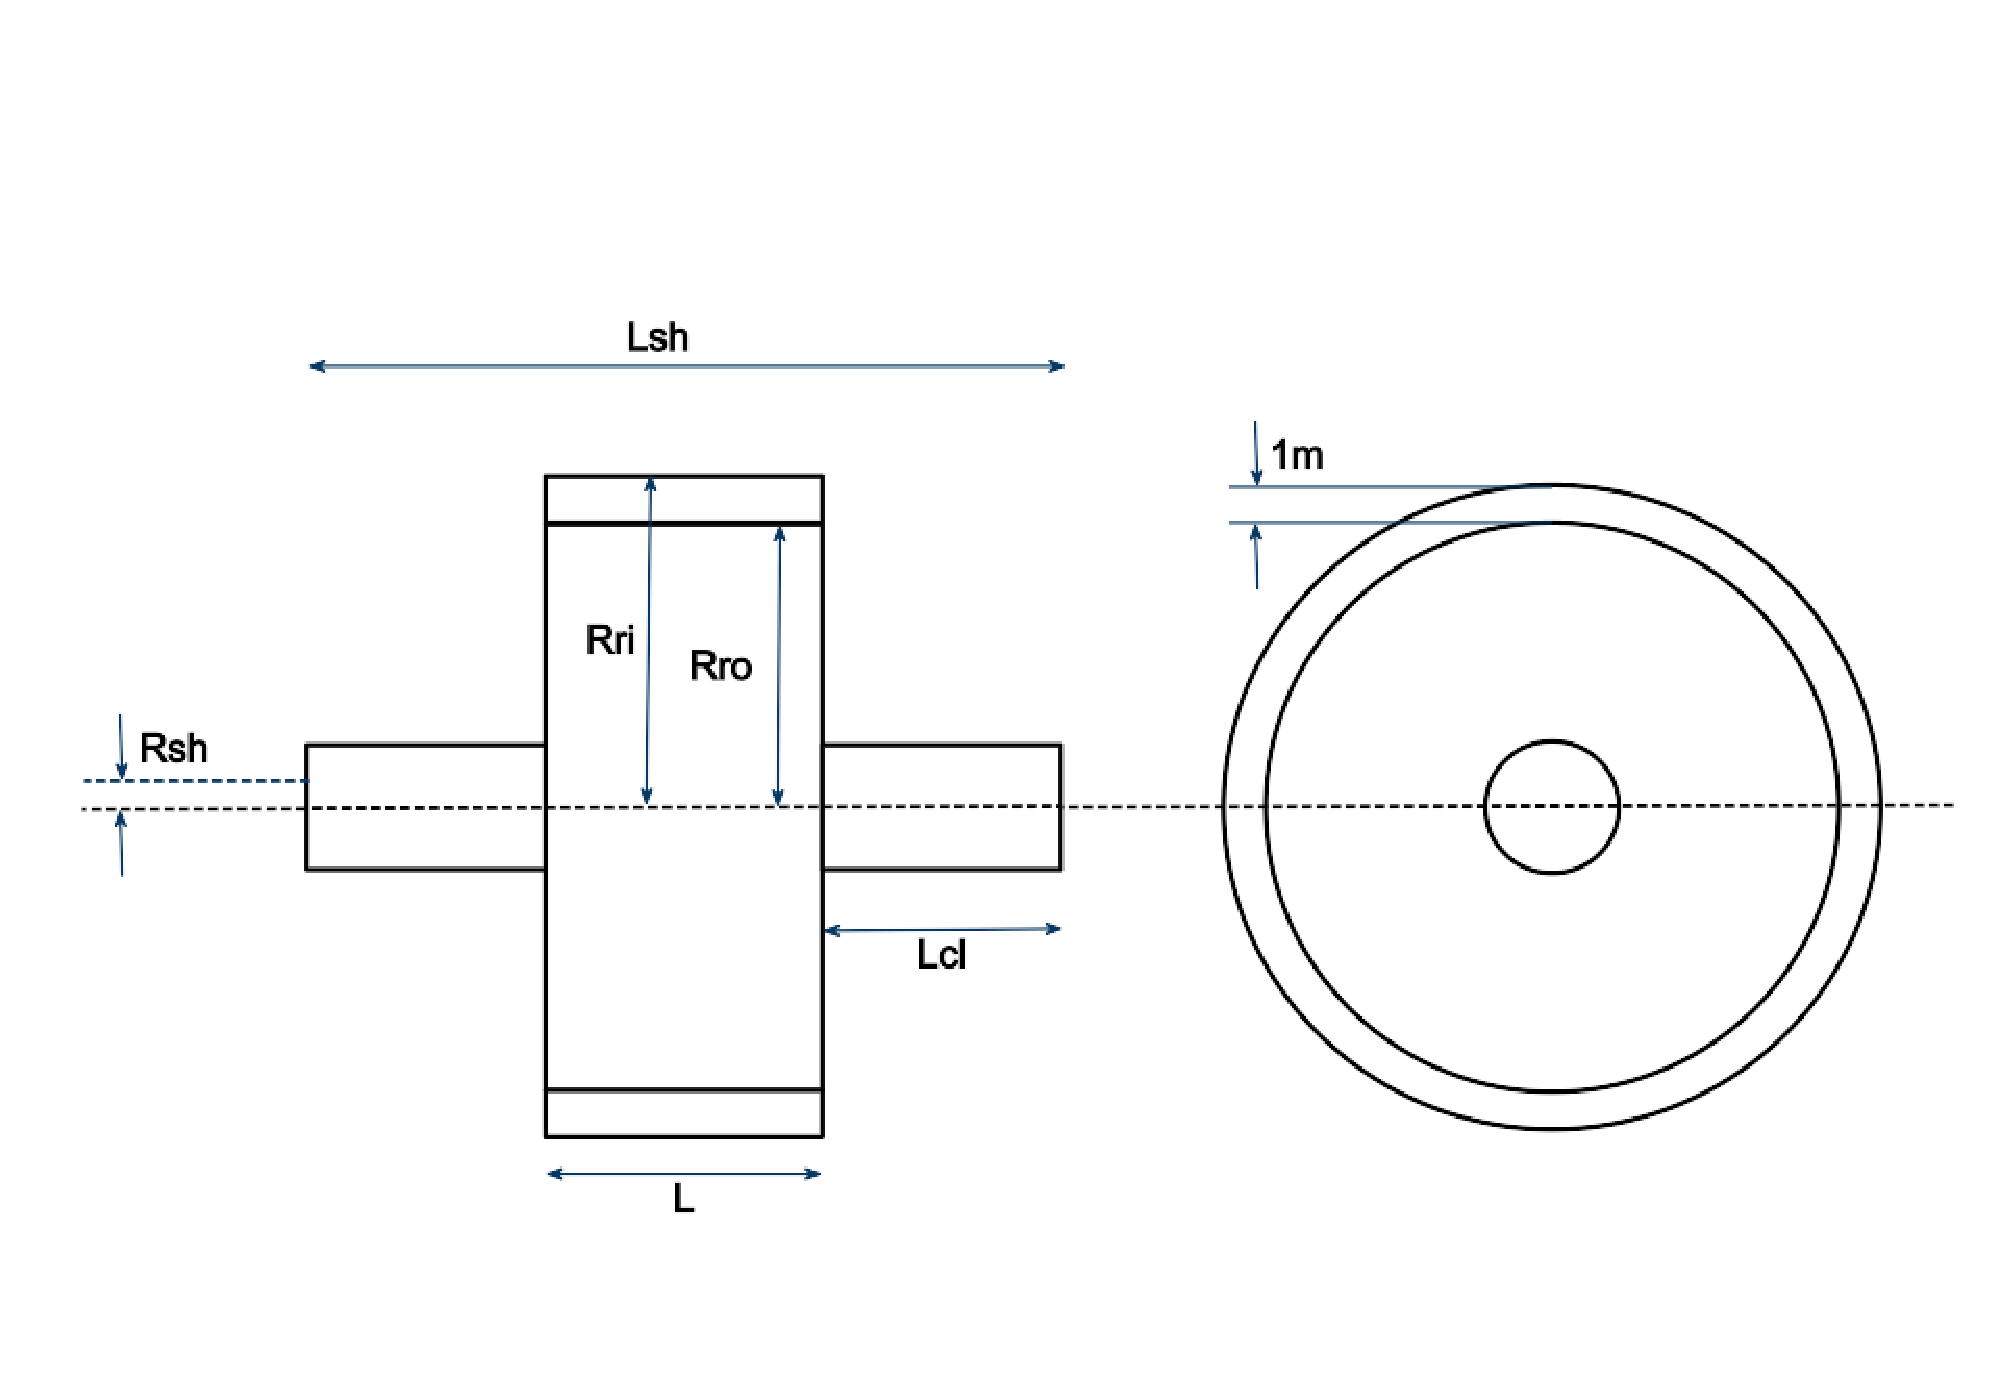
\includegraphics[width=80mm, height=59mm]{diagrams/bdcpmRotor.eps}}
 \caption{BDCPMM Rotor Assembly}
 \label{bdcpmRotor}
\end{center}\end{figure}

Five design variables are considered for the design process, other 
design parameters are fixed to values that are convenient for the 
manufacturer. The design variables are:

\begin{enumerate}
\item Number of laminations $n_l \in [44, 45,\dots ,132]$

\item Number of turns in each coil  $N \in [20, 21, \dots, 80]$

\item $L_{type} \in [\textsf{X, Y, Z}]$ is one of the three types of 
laminations allowed to build the motor

\item $M_{ph} \in [Y, \Delta ]$ is one of the two types of elctric 
connections and

\item $A_{gauge} \in [16, 16.5, 17, \dots , 23.5]$ is one of the 16 
wire gauges used in the windings.
\end{enumerate}

All the design variables are discrete in nature, of which $L_{type}$ 
and $M_{ph}$ take 3 and 2 values respectively. $n_l$ and $N$ are 
integer valued variables while $A_{gauge}$ takes 16 equally spaced 
values in its domain.

The cost expression for the first objecive includes the material and
estimated production cost. Each term in the expression is obtained 
from the regression analyses of data obtained from practice. The 
detailed procedure discribing the derivation of the cost terms and 
torque expressions can be found in \cite{chidambaram1999}.

The actual multi-objective optimization problem is formulated as 
follows:

%%%%%Cost function begins here%%%%%


\begin{singlespacing}

\begin{flushleft}



Minimize   \\
$ C_{total} (n_{l}, N, L_{type}, M_{ph}, A_{wire}) = 
\begin{cases}
\quad 2.6(\frac{n_{l}}{44})^{0.25}, & \text{for $L_{type} =$ X} \\
\quad 0.38 + 2.42(\frac{n_{l}}{44})^{0.37}, & \text{for $L_{type} =$ Y} \\
\quad 1.07 + 1.83(\frac{n_{l}}{44})^{0.58}, & \text{for $L_{type} =$ Z} 
\end{cases} $ \\

$
+  [ \left\{0.026, 0.028, 0.03\right\}n_{l} \cong L_{type} = \{ \textbf{X}, \textbf{Y}, \textbf{Z} \} $\\
$
\, + \, \dfrac{n_{l}}{44} \, + \,   9.8 \times 10^{5} A_{wire} N [ 5.8  \times  10^{-4} n_{l}
   +  \dfrac{\pi}{2} \{ w_{tb} + \dfrac{5\pi}{12}(R_{si} + \dfrac{d_{3}}{2}) \}]
$ \\

$
+ \, 0.3035 \, + \, 0.876 N [ 5.8 \times 10^{-4} n_{l} \, + 
 \dfrac{\pi}{2} \{ w_{tb} \, + \, \dfrac{5 \pi}{12}(R_{si} \, + \, \dfrac{d_{3}}{2})\}]
$\\

$
\, + \, \pi \left[ \left\{ 31.2( R_{si} + d_{3} + w_{bi}) + 0.0312 \right\} \left\{ L_{sh} - 5.08 \times 10^{-3} \right\} \right]
$\\
$
\, + \, 
\begin{cases}
\quad 0.7(\frac{5.8 \times 10^{-4} n_{l} + 0.0792}{0.1047})^{1.21},  & \text{for $L_{type} = $ X} \\
\quad 0.54 + 0.26( \frac{5.8 \times 10^{-4} n_{l} + 0.0802}{0.1057})^{3.74}, & \text{ for $L_{type} =$ Y} \\
\quad 0.58 + 0.32( \frac{5.8 \times 10^{-4} n_{l} + 0.0905}{0.1160})^{4.23}, & \text{ for $L_{type} =$ Z} \\
\end{cases}
$\\
$ \, + \, 9 \, + \, \begin{cases}
\quad 1.3(\frac{5.8 \times 10^{-4} n_{l} + 0.0792}{0.1047})^{0.38} (\frac{n_{l}}{44})^{0.18}, & \text{for $L_{type} =$ X} \\
\quad 1.6(\frac{5.8 \times 10^{-4} n_{l} + 0.0802}{0.1057})^{0.38} (\frac{n_{l}}{44})^{0.40}, & \text{for $L_{type} =$ Y} \\
\quad 1.8(\frac{5.8 \times 10^{-4} n_{l} + 0.0905}{0.1160})^{0.41} (\frac{n_{l}}{44})^{0.52}, & \text{for $L_{type} =$ Z}
\end{cases}
$\\
$
\, + \, (1.536 R_{st} - 6.26 \times 10^{-3}) n_{l} \, + \, (2.014 R_{si} \, - \, 8.21 \times 10^{-3}) n_{l}
$\\
$
\, + \, \pi \{29.4(R_{si} - 7.25 \times 10^{-3})^{2} n_{l} \, + \, 1.014 \times 10^{5} R_{sh}^{2} L_{cl}\} 
$\\
$
\, + \, 0.1862 \, + \, 5.31 \times 10^{4} \pi [ R_{st}^{2} L_{st} \, - \,  2 R_{sh}^{2} L_{cl} 
\, - \, 5.8 \times 10^{-4} n_{l}(R_{si} - 7.25 \times 10^{-3})^{2}] 
$\\
$
 \, + \, 0.01 \, + \,0.1473 \pi (R_{si} - 7.25 \times 10^{-3}) n_{l} \, + \, \begin{cases}
\quad 1.2, & \text{for $T_{p} \le 3.5$} \\
\quad 1.6, & \text{for $T_{p} > 3.5$} 
\end{cases}
$\\
$
\, + \, \left[ \left\{ 0.5, 0.55, 0.60 \right\} \cong L_{type} = \{ \textbf{X}, \textbf{Y}, \textbf{Z} \} \right]
$\\
$
\, + \, \begin{cases}
\quad 3.2(\frac{5.8 \times 10^{-4} n_{l} + 0.0792}{0.1047})^{-1.92}(\frac{n_{l}}{44})^{0.92}, & \text{for $L_{type} = $ X} \\ 
\quad 3.4(\frac{5.8 \times 10^{-4} n_{l} + 0.0802}{0.1057})^{-1.92}(\frac{n_{l}}{44})^{1.06}, & \text{for $L_{type} = $ Y} \\ 
\quad 3.7(\frac{5.8 \times 10^{-4} n_{l} + 0.0905}{0.1160})^{-3.25}(\frac{n_{l}}{44})^{1.60}, & \text{for $L_{type} = $ Z} 
\end{cases}
$
\\[\baselineskip]

%%%%Torque function%%%%

Maximize \\
$ T_p = 87300 C_{tor} N R_{si} A_{wire} n_{l} $\\
where \\
$ C_{tor} = \{ \frac{2}{3}, \frac{1}{3} \} \cong M_{ph} = \{ \textbf{Y}, \Delta  \} $ 
\\[\baselineskip]


Subject to \\
$g_1: T_{p} \geqslant 0.83$ \\

$g_2: T_{p} \leqslant 5.27$ \\

$g_3: A_{wire}N \leqslant \{150, 240, 280\} \times 10^{-7} \cong L_{type} = \{ \textbf{X}, \textbf{Y}, \textbf{Z} \}$

\end{flushleft}

\end{singlespacing}

Constraints $g_1$ and $g_2$ bound the peak torque in the desired 
range. Constraint $g_3$ represents the winding constraints that 
prevent magnetic saturation and demagnetization.

\subsubsection{NSGA-II formulation and the pareto-front}
Since all the variables are discrete, we use binary representation
for them in NSGA-II. We modify the population initialization routine
and the EA operators (recombination and mutation) to maintain the 
discrete nature of the variables. For the two integer valued 
variables, $n_l$ and $N$, discrete version of the Simulated Binary 
Crossover (SBX) and Polynomial Mutation \cite{deb2001} are used. Since
$M_{ph}$ and $L_{type}$ take two and three values only, they are only
subjected to mutation. Using this representation NSGA-II yeilds 199 
non-dominated solutions, plotted in figure \ref{nsplsp} in red circles.


\begin{figure}[ht]\begin{center}
 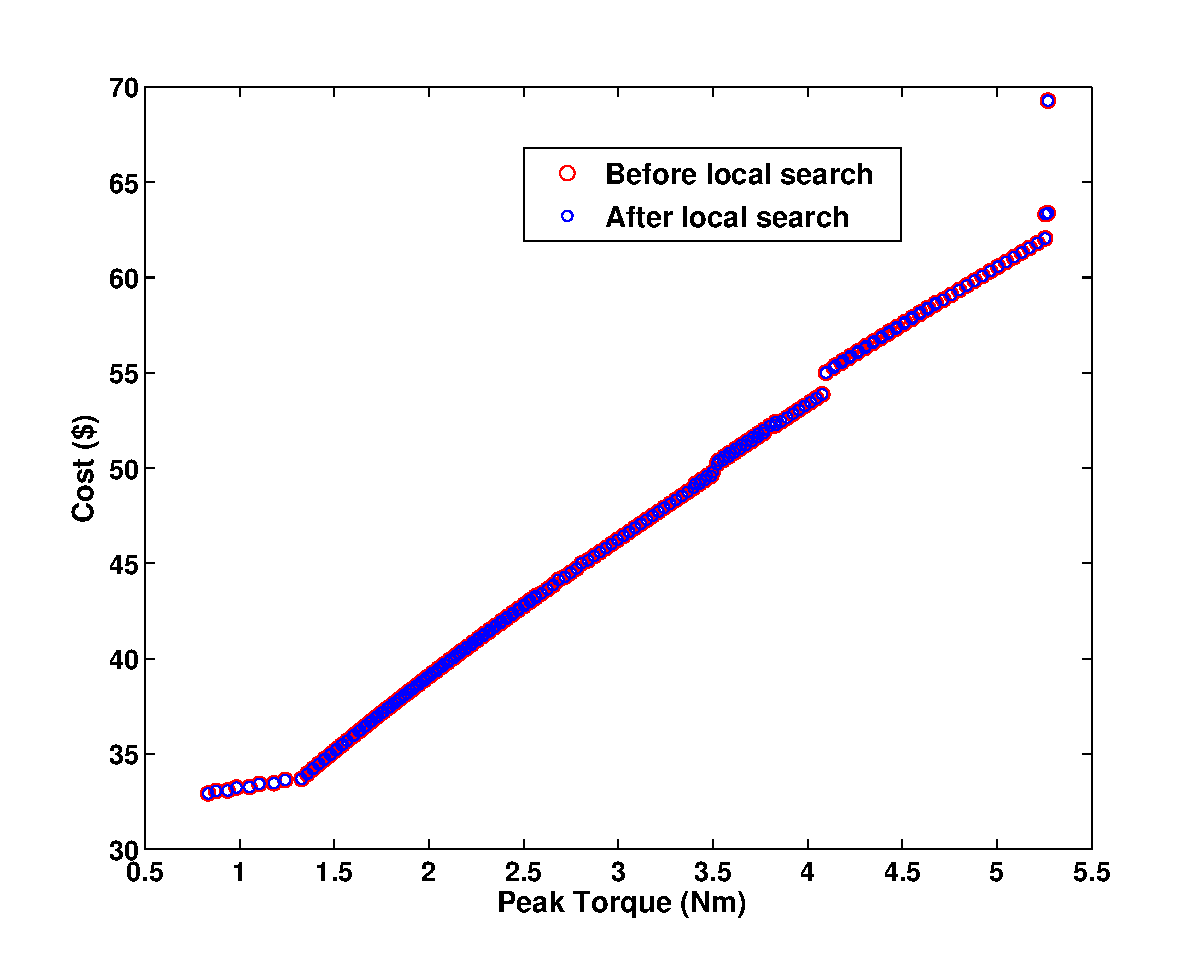
\includegraphics[width=90mm, height=75mm]{diagrams/nsplsp.eps} 
 \caption{Pareto-front for the BDCPMM design problem}
 \label{nsplsp}
\end{center}\end{figure}


\subsection{Local search procedure}
Although an evolutionary procedure may find a set of near optimal 
solutions quickly, the convergence to the true pareto-front might take 
indefinitely long. To improve convergence characteristics of the 
evolutionary multi-objective algorithms they are often complemented with
a local search procedure. Local search is more important in case of 
multi-objective optimization problems which invole discrete variables.
We have used a generic local search procedure which evaluates random 
solutions in the vicinity of the near-optimal solution under 
consideration. other optimization problems as well. The input for 
local search are the set of near optimal solutions $S$, number of 
local search iterations to perform $n$ , number of local solutions to 
evaluate for each near optimal solution $h$, and the search width 
factor $\sigma$. The algoritm \ref{localsearch} gives the algorithm 
for for our local search procedure.

\begin{algorithm}
\SetKwInOut{Input}{input}\SetKwInOut{Output}{output}
\Input{A set of near optimal solutions $S$,\\
number of itereations toperform $n$,\\
number of nearest neighbors to consider,\\
number of solutions to evaluate for each solution in $S$, $h \quad \forall s \in S $,\\
Scaling factor $\sigma$}
\Output{Set of optimal solutions $P$}
$P = \phi$;\\
\For{$i = 0$ to $n$}{
\For{each $s \in S$}{
add $s$ to $P$;\\
find $k$ nearest neighbors of $s$;\\
find the range of values each variable takes in the $k$-neighborhood;\\
\For{$j = 0$ to $h$ }{
generate a candidate random solution $p$ having variable values in the 
neighborhood range scaled by $\sigma$;\\
add $p$ to $P$;
}
}
perform non-dominated sorting on $P$ and discard dominated solutions;\\
$S$ = $P$;
}
return $P$;
\BlankLine
\caption{Local search procedure}
\label{localsearch}
\end{algorithm}

For the BDCPMM design problem, however, local search doesn't result in 
much improvement since we ran NSGA-II for a large number of 
generations(3000) which would have been sufficient for convergence to
the actual pareto-front. Performing local search on the NSGA-II output
for BDCPMM design problem increases the number of optimal solutions 
to 201 from 199.

\section{Learning chunks from the optimal solutions (Estimating the pareto-front manifold}
If $k$ conflicting objectives have to be optimised simultaneously in 
a multi-objective optimization, the resulting pareto-front would be a 
$k-1$ dimensional manifold in the obejctive space. Modelling the 
pareto-front as a manifold may reveal how the objectives are related 
to each other, whether they are mutually conflicting in that case we 
will get a $k-1$ dimensional manifold, or some of them vary direclty 
with each other then the manifold will be of dimension less than $k-1$.
Similarly a linear dimensionality reduction analasys may reveal the 
relative importance of the design variables.
  
In \cite{mukerjee2009} a frame work for learning design symbols 
using non-linear manifold learning is presented. However, as we shall 
see, the pareto-fronts in real design instances might not be a single 
continuous manifold, instead they might consist of many desparate 
clusters of related designs. Learning these clusters as specialized 
chunks of optimal designs may be more useful than simply learning 
pareto-front as a manifold. In this section we present a procedure for
clustering the optimal solutions and learning these as specialized 
chunks.

\subsection{Estimating intrinsic dimensionality of the pareto-front using Isomap}
Manifold learning algorithms are based on the basic assumption that
the data is embedded in a single low-dimensional continuous manifold.
These algorithms can thus be used to estimate the intrinsic 
dimensionality of the optimal sets. We use Isomap residual variance
to estimate the intrinsic dimensionality of the pareto-front. 
Similarly, an analysis of the PCA explained variance may reveal which 
are the parameters that vary in optimal designs.

\subsubsection{Isomap Residual Variance for the Pareto-front}
On performing Isomap on the pareto-front data of BDCPMM design we 
obtain a residual variance plot shown in figure \ref{isoRVbdcpmAll}. 
Since the residual variance shows a sharp decline going from one 
dimensional embedding to two-dimensional embedding, we can expect the 
pareto-front to be composed of sub-manifolds of one or two dimensions.
There is an unexpected increase in the residual variance for three 
dimensional embedding, though it drops down to the previous level for 
four dimensional embedding. 

\subsubsection{PCA explained variance}
The PCA analysis of BDCPMM pareto-front gives four principal 
components.  The explained variance for 
principal components of the BDCPMM pareto-front data are plotted in 
figure \ref{pcaEVbdcpmAll}. The first principal component has 
explained variance of more than 0.95, while the second principal 
component has explained variance of 0.021. The third and fourth 
principal components have negligible explained variances. Table 
\ref{firstTwoPCs} shows the three principal component vectors which 
reveal that the pareto front is a manifold embedded in the plane of 
first two design dimensions, namely number of laminations and number 
of turns in the stator windings.
 
\begin{figure}[ht]\begin{center}
 \subfloat[Isomap Residual Variance for the Pareto-front]{
 \label{isoRVbdcpmAll} \includegraphics[width=62mm, height=52mm]{diagrams/isoRVbdcpmAll.eps}}
 \subfloat[Explained variance for Principal Components of the Pareto-front]{
 \label{pcaEVbdcpmAll} \includegraphics[width=62mm, height=52mm]{diagrams/pcaEVbdcpmAll.eps}}
 \caption{Isomap and PCA results}
 \label{bdcpmmVar}
\end{center}\end{figure}

\begin{table}[!ht]
\centering
\begin{tabular}{|c|c|c|c|c|c|}
 \hline
 First PC & 0.9993 & 0.0370 & 0.0072 & 0 & -0.0024\\
 \hline
 Second PC & -0.0367 & 0.9943 & 0.0165 & 0 & 0.0985\\
 \hline
 \end{tabular}
\caption{First two principal components of the BDCPM data}
\label{firstTwoPCs}
\end{table}


\section{Clustering the pareto-front}

\begin{algorithm}
\SetKwInOut{Input}{input}\SetKwInOut{Output}{output}
\Input{($D$, $c_t$, $n_{max}$, $k_g$, $k_l$)}
\Output{A cluster labelling for each data-point}
\BlankLine
find $n_{max}$ nearest neighbors of each point arranged in non-decreasing
order of the distance;\\
$ad_{g} =$ average interpoint distance in the data set;\\
${\sigma}_g =$ standard deviation of distances in the dataset;\\
$G =\{V, E\}$ be a graph where $V$ is the set of all datapoints and $E = \phi$;\\ 
\For{$i = 1$ to $n_{max}$}{
\For{each connected component $c$ in $G$}
{
find out the average and standard deviation of edge weights in $c$;\\
}
\For{each point $p$ in the data set}
{
\If{ $p$'s nearest neighbor list is empty}
{
continue;\\
}
$csize =$ no. of points in the connected component $p$ belongs to;\\
    \eIf{$csize \leqslant c_t$}
    {
      $q =$ the first point in the nearest neighbor list of $p$;\\
      $d =$ distance to first point in ordered nearest neighbors list of $p$;\\
      \eIf{$d > ad_g + k_g {\sigma}_g$}
      {
        \tcc{if $i = 0$ then $p$ is an outlier}
        remove all points from the ordered nearest neighbors list of $p$;\\
      }
      {
        \If{ $(q, p) \notin E$}
        {
          add ($p$, $q$) to $G$;\\
          remove $q$ from ordered nearest neighbors list of $p$;\\
        }
      }
    }
    {
      \eIf{$d > ad_c + k_l {\sigma}_c$}
      {
        \tcc{no further connections from $p$}
        remove all points from the ordered nearest neighbors list of $p$;\\
      }
      {
        \If{ $(q, p) \notin E$}
        {
          add ($p$, $q$) to $E$;\\
          remove $q$ from ordered nearest neighbors list of $p$;\\
        }
      }
    }
  }
}
\caption{Clustering algorithm to obtain low-dimensional clusters}
\label{clusteralgo}
\end{algorithm}



\subsection{Clusters in the BDCPMM pareto-front}
The clustering of the BDCPMM pareto-front results in five clusters 
which are shown in the objective space plot in figure \ref{bClustersO}. 
Figure \ref{bClustersP} shows the clusters with respect to the number
of laminations and the Wire Gauge used in the stator windings. Other  
design variables are indicated alongside the clusters.

\begin{figure}[ht]\begin{center}
 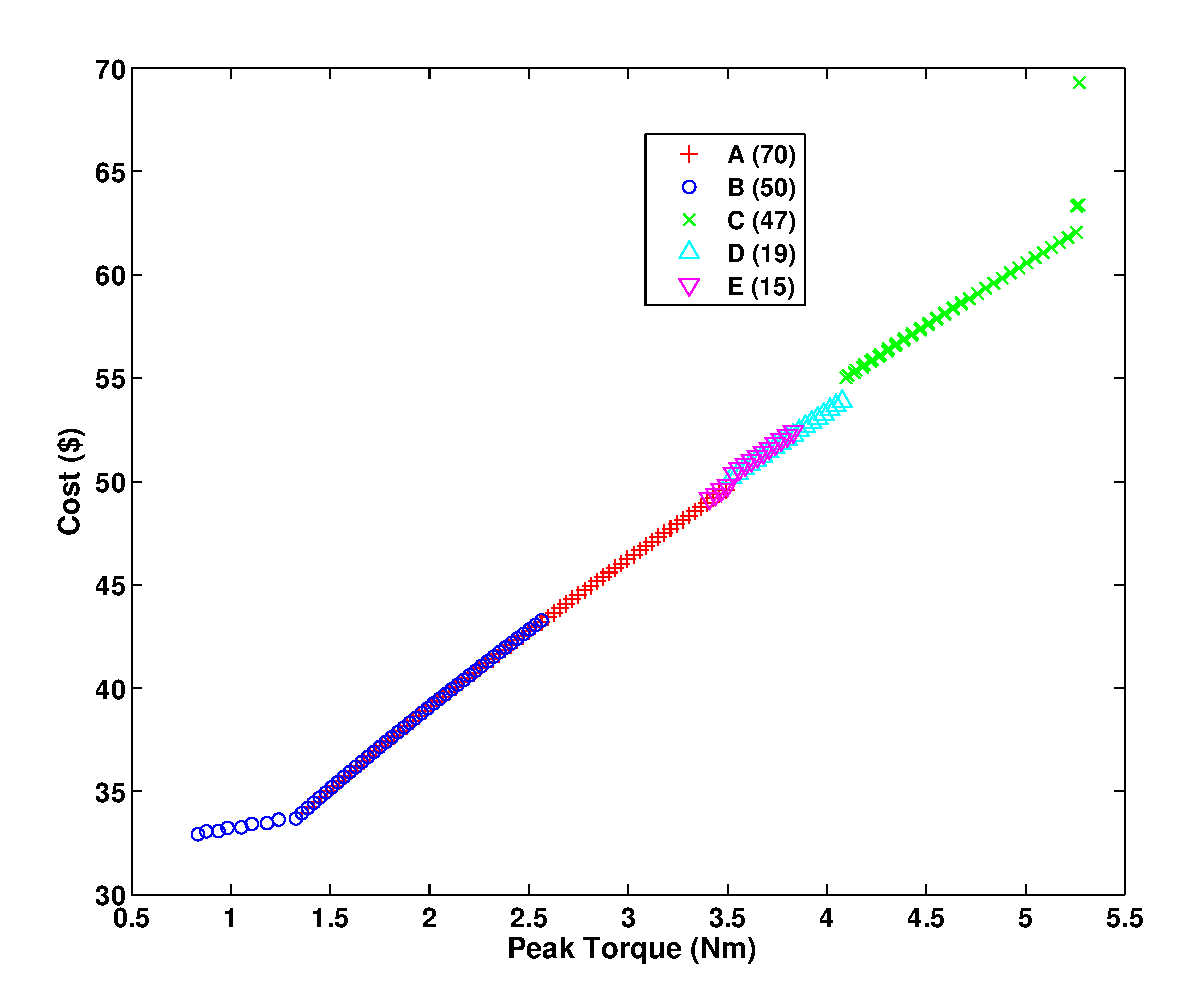
\includegraphics[width=100mm, height=80mm]{diagrams/bClustersO3.eps} 
 \caption{Clusters in the BDCPMM pareto-front}
 \label{bClustersO}
\end{center}\end{figure}

\begin{figure}[ht]\begin{center}
 \includegraphics[width=100mm, height=80mm]{diagrams/bClustersP2.eps} 
 \caption{Clusters in the \#Laminations-Wire-gauge subspace.}
 \label{bClustersP}
\end{center}\end{figure}
 

\section{What do the clusters represent (design implications of the chunks)}
Cluster \textbf{A} is the largest in terms of number of optimal 
solutions. It also has the largest torque range, from 1.35 Nm to 3.49
Nm. All the designs in this cluster have 23 turns in the stator 
windings. It  has significant overlap with cluster \textbf{B} in the 
objective space, though \textbf{B} has lower number of turns in the 
stator coil. This is possible because designs in \textbf{B} are using
a thicker wire in the stator windings which compensates for decrease 
in torque due to lower number of turns and also increases the cost to 
the level of designs in \textbf{A}.

\textbf{B} is the cluster of low end designs. The torque range for 
this cluster is 0.83 Nm to 2.56 Nm. For torque requirements in the 
range 1.35 Nm to 2.56, the designer can choose from either \textbf{A}
or \textbf{B}, depending on which design best meets the 
specifications. The designs in cluster have 20 or 21 turns in the 
stator windings, 20 for lower torque and cost and 21 for higher torque
and cost motors. 

 
Cluster \textbf{C} has the high end designs of motors. There are two 
overlapping pareto-fronts in the torque range 4.09 Nm to 4.71 Nm. That
means there are a larger number of optimal designs in this range. The
designs in this range alternate between 24 turns in the stator 
windings with 16 gauge wire and 24 turns with 16.5 gauge wire. These 
alternations are visible in the figure \ref{bClustersP} in the form of
two lines of upward pointing triangles at Wire Gauge values of 16 and
16.5. One thing that sets apart these designs from all others is that 
they all use lamination type Z whereas all others use lamination type 
Y. This implies that Z type laminations are useful only for high end
motors.

Clusters \textbf{D} have \textbf{E} overlaps similar to clusters 
\textbf{A} and \textbf{B} with \textbf{E} covering the lower torque 
range. 


These clustering results of the BDCPMM pareto-front illustrates 
results of a single multi-obejctive optimization may result in 
desparate interrelated chunks.
